\chapter{Stand der Technik}
\section{Getränkemischmaschine}
\section{Hardware}
\section{Sprachverarbeitung}
\subsection{Spracherkennung}
\subsection{Vergleich verschiedener Ansätze}
Derzeit gibt es vier Hauptansätze für die Erstellung eines Chatbots:
\begin{itemize}
    \item Musterabgleich - Musterabgleich und Antwortvorlagen (vorgefertigte Antworten)
    \item Grounding - logische Wissensgraphen und das Ziehen von Schlussfolgerungen aus diesen basierend auf diesen Graphen
    \item Suche - Abrufen von Text
    \item Generierungsmethoden - Statistik und maschinelles Lernen.
\end{itemize}
Die vier grundlegenden Ansätze zur Erstellung von Chatbots lassen sich kombiniert werden, was zu benutzerfreundlichen Chatbots führt. Viele Vielzahl von Anwendungen nutzen alle vier grundlegenden Methoden. Hybride Chatbots unterscheiden sich hauptsächlich darin, wie genau sie diese Ansätze kombinieren und wie viel Gewicht auf jeden einzelnen Ansatz gelegt wird.
\subsubsection{Musterabgleich}
Bei den ersten Chatbots basierte die Antwort auf die Nachricht eines Benutzers auf einem Mustervergleich. Diese Chatbots suchen nach Mustern im eingehenden Text und geben eine feste (gemusterte) Antwort, wenn eine Übereinstimmung gefunden wird (//BUCH).\\\\
Solche rudimentären Dialogsysteme sind vor allem in automatisierten Benutzerunterstützungssystemen mit interaktiven Sprachmenüs nützlich, wo es möglich ist, das Gespräch an einen Menschen weiterzuleiten, wenn der Chatbot keine Antwortmuster mehr hat.\\\\
Da es viele NLP-Dienstprogramme in Python-Paketen gibt, ist es möglich, komplexere Chatbots auf der Grundlage von Mustervergleichen zu erstellen, indem man die Bot-Logik nach und nach direkt in Python mit regulären Ausdrücken und Suchmustern aufbaut.\\\\
1995 machte sich Richard Wallace daran, einen allgemeinen Rahmen für die Erstellung von Chatbots auf der Grundlage des Pattern-Matching-Ansatzes zu schaffen. Zwischen 1995 und 2002 schuf seine Entwicklergemeinschaft die Artificial Intelligence Markup Language (AIML) zur Beschreibung von Mustern und Chatbot-Antworten.\\\\
AIML ist eine deklarative Sprache, die auf dem XML-Standard basiert, der die Sprachkonstrukte und Datenstrukturen einschränkt, die im Bot verwendet werden dürfen. Ein Chatbot, der auf AIML basiert, sieht folgendermaßen aus:
\begin{figure}[H]
    \centering
    \fbox{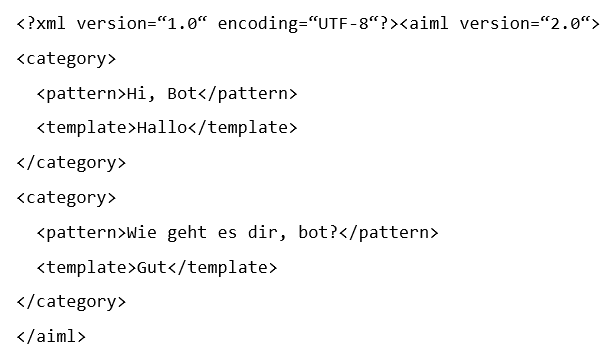
\includegraphics[width=0.8\textwidth]{Bilder_Kapitel_2/aiml_bot.png}}
    \caption{\label{figure:Aiml_Bot}AIML Chatbot}
\end{figure}
\noindent
Eine der Einschränkungen von AIML ist die Art der Muster, die abgeglichen werden können und auf die reagiert wird. Der AIML-Kern (Pattern Matching Engine) reagiert nur auf Eingabetext, der einem vom Entwickler manuell vorgegebenen Muster entspricht. Unscharfe Suchanfragen, Smileys, Satzzeichen, Tippfehler oder falsch geschriebene Wörter sind nicht erlaubt, es findet kein automatischer Abgleich statt. In AIML müssen alle Synonyme manuell einzeln beschrieben werden.
\subsubsection{Grounding}
Die Grounding-Methode ist ein Ansatz zur Erstellung eines Chatbots auf der Grundlage logischer Wissensgraphen und der Durchführung von Schlussfolgerungen auf der Grundlage dieser Graphen. Sie wird verwendet, um natürliche Sprache zu verarbeiten und sie dem Verständnis des Bots zuzuordnen. Das Wesentliche an der Grounding-Methode ist, dass der Chatbot nicht nur die Textnachrichten, sondern auch den Kontext und die Umgebung verarbeitet, um Anfragen besser zu verstehen und zu beantworten. Durch die Extraktion von Informationen wird ein Netz von Verbindungen oder Fakten geschaffen. Dieses Netz logischer Verbindungen zwischen Entitäten - ein Graph oder eine Wissensbasis - kann die Grundlage für die Antworten des Chatbots bilden.\\\\
Ein Beispiel für eine Grounding-Methode ist die Verwendung eines Wissensgraphen zur Beschreibung der Umgebung. Ein Wissensgraph enthält Informationen über die Objekte, mit denen der Bot interagieren kann, und die Beziehungen zwischen ihnen. Ein Wissensgraph könnte zum Beispiel Informationen über ein Glas auf einem Tisch und das darin befindliche Wasser enthalten. Wenn ein Benutzer eine Frage stellt, verwendet der Chatbot den Wissensgraphen, um den Kontext der Anfrage zu verstehen und die am besten geeignete Antwort abzuleiten. Wenn ein Benutzer zum Beispiel fragt: "Wie hoch ist die Temperatur des Wassers in dem Glas auf dem Tisch?", kann der Chatbot Informationen aus dem Wissensgraphen verwenden, um die Frage zu beantworten.\\\\
Ein solcher Wissensgraph kann abgeleitet werden, um Fragen über die in dieser Wissensbasis enthaltene Welt zu beantworten, und dann können auf der Grundlage der logischen Antworten die Werte der in den Antworten enthaltenen Template-Variablen ausgefüllt werden, um natürlichsprachliche Antworten zu erstellen. Ursprünglich wurden auf diese Weise Systeme zur Beantwortung von Fragen eingerichtet, wie z. B. der Watson-Bot von IBM (heutzutage wird für ähnliche Systeme jedoch die Information Suche Methode verwendet). Der Wissensgraph stellt eine Art 'Erdung' des Chatbots in der realen Welt dar.\\\\
Die Erstellung von Chatbots auf der Grundlage von "Grounding" eignet sich hervorragend für Chatbots, die Fragen generieren, bei denen das zur Beantwortung einer Frage erforderliche Wissen in einer umfangreichen Wissensbasis enthalten ist, die aus einer offenen Datenbank (z. B. Wikidata, Open Mind Common Sense oder DBpedia) bezogen werden kann.\\\\
Einer der Hauptvorteile der Grounding-Methode besteht darin, dass sie sich an ein sich veränderndes Umfeld anpassen kann. Wenn der Benutzer zum Beispiel ein Glas Wasser von einem Tisch auf einen anderen stellt, wird der Wissensgraph automatisch aktualisiert, um diese Änderung widerzuspiegeln.\\\\
Grounding-Methode hat jedoch auch ihre Grenzen. Sie kann bei der Verarbeitung großer Informationsmengen und dadurch eingeschränkt sein, dass sie Zusammenhänge nicht berücksichtigt, die dem Bot möglicherweise verborgen bleiben.\\\\
Insgesamt ist die Grounding-Methode ein effektiver Ansatz zur Erstellung wissensbasierter Chatbots. Sie ermöglicht es dem Bot, Benutzeranfragen besser zu verstehen und eine genauere Antwort zu geben.
\subsubsection{Suche}
\subsubsection{Generierungsmethoden}
\endinput